\chapter{Conclusion}

In this chapter, we summarize our contributions in the thesis and present some
future extensions.
% - Recall contributions with more details assuming someone has read it
%
% - Future work (chapter by chapter)
\section{Contributions}

In this thesis, we have developed some tools to better understand and make use
of the computations happening within complex systems.
We summarize our contributions below.

\begin{itemize}
  \item In Chapter \ref{cha:background}, we gave an overview of the \acf{CA}
        model and the specific challenges it poses. We review the deep
        connection between \acp{CA} and \acfp{RNN} and how this leads to using
        \acp{CA} in \acf{RC}. Next, in chapter \ref{cha:literature-review}, we
        place our work within the large body of literature on complex systems,
        complexity, emergence and learning.

  \item In Chapter \ref{cha:meas-compl-evolv}, we define a novel metric of
        complexity for complex systems. The metric is inspired by principles of
        compression, and algorithmic complexity. It uses the ability of small
        neural networks to learn a model of the local structures in a system,
        and the evolution of the predictive power of that model as the system
        evolves over time. We evaluate the quality of this metric by measuring
        its correlation with the perception of complexity of humans. We find a
        higher correlation with human annotations than alternative methods on a
        dataset of \acp{CA} rules labeled as complex or not. We use the metric
        to discover new \acp{CA} rules with surprisingly complex behavior
        semi-automatically.

  \item In Chapter \ref{cha:visu-comp-large}, we built on the work of Chapter
        \ref{cha:meas-compl-evolv} to work on the specific challenges posed by
        working with large-scale systems such as cellular automata. In these
        systems, qualitatively different behavior may emerge at various scales.
        To allow dealing with these large systems and apply complexity measures
        and classification methods on a range of scales, we developed three
        coarse-graining methods based on simple statistical analysis, clustering
        algorithms and autoencoder neural networks, that can reduce the size of
        a system while retaining useful information.

  \item In Chapter \ref{cha:learn-effic-compl}, we tackled the issue of using
        complex systems for general purpose task solving, using the \ac{RC}
        paradigm. We also developed a metric for the speed of learning of
        machine learning systems. Using that metric, we looked at the data
        efficiency of some well know algorithms rather than their task-based
        performance only. Surprisingly, \ac{RC} models using random frozen
        \acp{RNN} or \acp{CA} are significantly more efficient that other
        alternatives on a range of tasks. We evaluated this on some standard
        language datasets and introduced our own dataset of progressively more
        complex tasks. Efficiency is a crucial property in low data and compute
        settings, and our work showed that some overlooked methods may actually
        be competitive in these situations.
\end{itemize}

\section{Future Work}

\subsection{Evolving cellular automata for complexity}

The metric of complexity developed in Chapter \ref{cha:meas-compl-evolv} and the
others presented in Section \ref{sec:measuring-complexity} often give a single
value output from a system's evolution over time. Similar to how
\textcite{mitchellEvolvingCellularAutomata1996} evolves \acp{CA} rules to solve
a particular task, it seems appealing to use the complexity as a fitness
function for a genetic algorithm. Such an algorithm would generate new rules
that are progressively more complex (according to the complexity metric).

It is hard to apply this principle in practice,


\subsection{Feedback reservoir computing}

In Chapter \ref{cha:learn-effic-compl}, we explored the applications of the
\ac{RC} paradigm to \acp{CA}. In general, \ac{RC} assumes a purely forward
model, meaning that inputs are fed to the reservoir and outputs are decoded from
it. The trainable decoder layer is trained offline on a training dataset and
tested next. We illustrate the \ac{RC} principle in figure
\ref{fig:classical_reservoir}. This structure is often sufficient for supervised
tasks when a sufficiently large training dataset is available.

\begin{figure}[htbp]
  \centering
  \begin{subfigure}[t]{.5\linewidth}
    \centering
    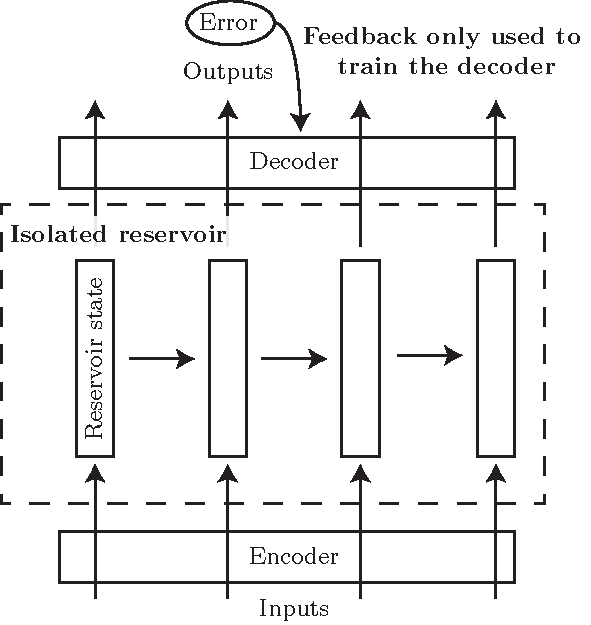
\includegraphics[width=\linewidth]{figures/classical_reservoir.pdf}
    \caption{Classical reservoir computing}
    \label{fig:classical_reservoir}
  \end{subfigure}
  \begin{subfigure}[t]{.45\linewidth}
    \centering
    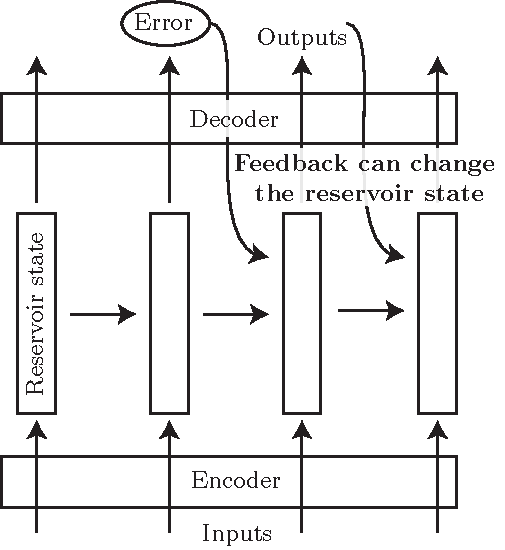
\includegraphics[width=\linewidth]{figures/feedback_reservoir.pdf}
    \caption{Feedback reservoir computing}
    \label{fig:feedback_reservoir}
  \end{subfigure}
  \caption{Comparison of regular reservoir computing with feedback reservoir computing}
  \label{"waiting for reftex-label call..."}
\end{figure}
